%=====================================================================
%  SHARED PREAMBLE — Quantitative Reasoning LAB 413 Beamer theme
%  Paste this block VERBATIM at the top of every LabN_beamer.tex
%  (keep each deck self-contained; do NOT \input this file).
%  Compile: pdflatex LabN_beamer.tex   (run twice for footline counters)
%=====================================================================
\documentclass[aspectratio=169,11pt]{beamer}

\usepackage[utf8]{inputenc}
\usepackage[T1]{fontenc}
\usepackage{lmodern}
\usepackage{amsmath,amssymb}
\usepackage{graphicx}
\usepackage{booktabs}
\usepackage{tcolorbox}
\tcbuselibrary{skins}

\usetheme{default}
\usecolortheme{default}
\useinnertheme{circles}

\definecolor{qrnavy}{RGB}{20,44,90}
\definecolor{qrblue}{RGB}{38,80,150}
\definecolor{qrgray}{RGB}{90,95,105}
\definecolor{qrlight}{RGB}{234,239,247}
\definecolor{qrred}{RGB}{190,60,60}

\setbeamercolor{structure}{fg=qrnavy}
\setbeamercolor{frametitle}{fg=white,bg=qrnavy}
\setbeamercolor{title}{fg=qrnavy}
\setbeamercolor{block title}{fg=white,bg=qrblue}
\setbeamercolor{block body}{bg=qrlight}
\setbeamercolor{itemize item}{fg=qrblue}
\setbeamercolor{itemize subitem}{fg=qrblue}
\setbeamerfont{frametitle}{series=\bfseries}
\setbeamertemplate{navigation symbols}{}

\setbeamertemplate{frametitle}{%
  \nointerlineskip
  \begin{beamercolorbox}[wd=\paperwidth,ht=3.2ex,dp=1.2ex,leftskip=0.3cm]{frametitle}%
    \strut\insertframetitle\strut
  \end{beamercolorbox}%
}

% Footline: course | lab N | slide number  (edit "Lab N" per deck)
\newcommand{\labnum}{Lab 4}   % <-- SET THIS to the lab number, e.g. \renewcommand{\labnum}{Lab 3}
\setbeamertemplate{footline}{%
  \leavevmode%
  \hbox{%
    \begin{beamercolorbox}[wd=.5\paperwidth,ht=2.4ex,dp=1ex,leftskip=.3cm]{author in head/foot}%
      \usebeamerfont{author in head/foot}\color{qrgray}\small Quantitative Reasoning -- LAB 413%
    \end{beamercolorbox}%
    \begin{beamercolorbox}[wd=.5\paperwidth,ht=2.4ex,dp=1ex,rightskip=.3cm]{title in head/foot}%
      \usebeamerfont{title in head/foot}\color{qrgray}\small\hfill \labnum \quad\insertframenumber\,/\,\inserttotalframenumber%
    \end{beamercolorbox}}%
}

% Number badge (01, 02, ...) used on concept slides:  \numbadge{01}
\newtcbox{\numbadge}{on line,boxsep=2pt,left=4pt,right=4pt,top=2pt,bottom=2pt,
  colback=qrnavy,colframe=qrnavy,fontupper=\bfseries\color{white},arc=2pt}

% Key-concepts callout:  \begin{keybox} ... \end{keybox}   or  \begin{keybox}[Scenario] ...
\newtcolorbox{keybox}[1][Key Concepts]{colback=qrlight,colframe=qrnavy,
  fonttitle=\bfseries,title={#1},coltitle=white,arc=2pt,left=4pt,right=4pt,
  top=3pt,bottom=3pt,boxrule=0.6pt}

%---------------------------------------------------------------------
%  Title data
%---------------------------------------------------------------------
\title{\bfseries Causation, Experimental Design \& Sampling}
\subtitle{Week 5 Recap \textbullet\ Lab 4}
\author{Instructor: Subin Na}
\institute{Quantitative Reasoning -- LAB 413}
\date{September 24, 2025}

\begin{document}

%---------------------------------------------------------------------
%  Title slide
%---------------------------------------------------------------------
{\setbeamertemplate{footline}{}
\begin{frame}
  \vfill
  {\color{qrgray}\small Quantitative Reasoning -- LAB 413}\\[0.6em]
  {\usebeamerfont{title}\color{qrnavy}\huge\bfseries Causation, Experimental\\[0.15em]Design \& Sampling\par}
  \vspace{0.4em}
  {\color{qrblue}\large Week 5 Recap \ \textbullet\ \ Lab 4}\par
  \vspace{1.6em}
  {\color{qrgray} Instructor: \textbf{Subin Na} \hfill September 24, 2025}
  \vfill
\end{frame}
}

%---------------------------------------------------------------------
%  Today's Plan
%---------------------------------------------------------------------
\begin{frame}{Today's Plan}
  \begin{columns}[T]
    \begin{column}{0.5\textwidth}
      \textbf{\color{qrnavy}1. Quick Recap}
      \begin{itemize}
        \item Sources of Data
        \item Causation vs.\ Correlation
        \item What is Causality?
        \item RCTs
      \end{itemize}
    \end{column}
    \begin{column}{0.5\textwidth}
      \phantom{\textbf{x}}
      \begin{itemize}
        \item Problems with Experiments
        \item Sampling
        \item Survey Cautions
      \end{itemize}
      \vspace{0.8em}
      \textbf{\color{qrnavy}2. RStudio Practice}
    \end{column}
  \end{columns}
\end{frame}

%---------------------------------------------------------------------
%  01 Sources of Data
%---------------------------------------------------------------------
\begin{frame}{\numbadge{01}\ \ Sources of Data: Overview}
  \begin{itemize}
    \item \textbf{Anecdotal data:} individual striking cases (often outliers, not representative).
    \item \textbf{Observational data:} existing data collected for other purposes.
    \item \textbf{Sample surveys:} collecting opinions from representative samples.
    \item \textbf{Experiments:} deliberately imposing treatments to measure causal effects.
  \end{itemize}
\end{frame}

%---------------------------------------------------------------------
%  02 Causation vs Correlation  (EMBED causal diagrams)
%---------------------------------------------------------------------
\begin{frame}{\numbadge{02}\ \ Causation vs.\ Correlation}
  \begin{keybox}[Key Problem]
    Association $\neq$ Causation. Three explanations for an $X$--$Y$ correlation:
  \end{keybox}
  \vspace{0.3em}
  \begin{columns}[T]
    \begin{column}{0.5\textwidth}
      \begin{itemize}\small
        \item \textbf{Direct causation:} $X$ causes $Y$.
        \item \textbf{Common response:} $Z$ causes both $X$ and $Y$.
        \item \textbf{Confounding:} $X$ causes $Y$, but $Z$ also affects $Y$ and correlates with $X$.
      \end{itemize}
    \end{column}
    \begin{column}{0.5\textwidth}
      \centering
      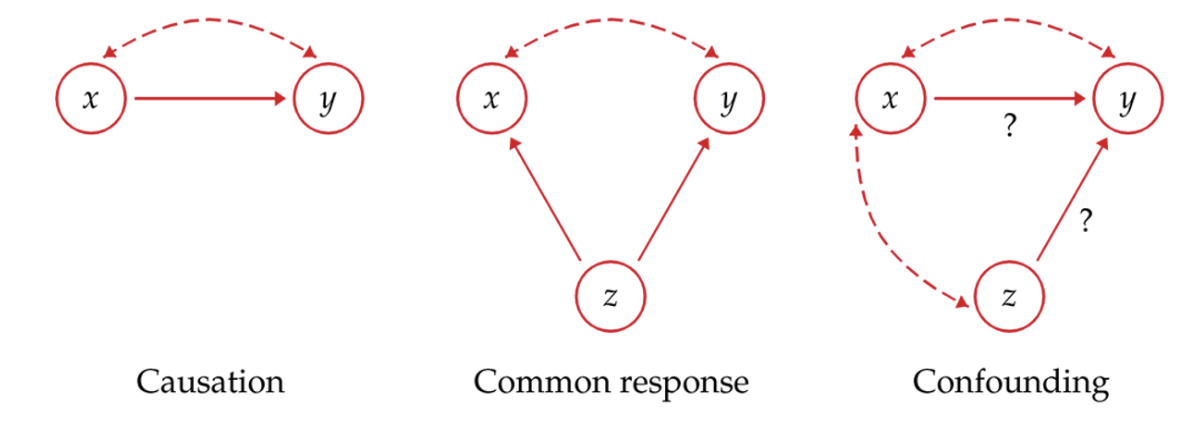
\includegraphics[width=\textwidth]{figures/s04_1_7.7x2.8.png}
    \end{column}
  \end{columns}
  \vspace{0.2em}
  \begin{center}\small
    \textbf{\color{qrnavy}Solution:} well-designed experiments can avoid confounding.
  \end{center}
\end{frame}

%---------------------------------------------------------------------
%  03 What is Causality?  (EMBED counterfactual figure)
%---------------------------------------------------------------------
\begin{frame}{\numbadge{03}\ \ What is Causality?}
  \begin{columns}[T]
    \begin{column}{0.58\textwidth}
      \begin{keybox}[Fundamental Problem]
        We can never observe counterfactuals.
      \end{keybox}
      \vspace{0.4em}
      \begin{itemize}
        \item \textbf{Factual:} what actually happened.
        \item \textbf{Counterfactual:} what would have happened otherwise.
      \end{itemize}
      \vspace{0.4em}
      \begin{equation*}
        \text{Causal Effect} = Y(1) - Y(0)
      \end{equation*}
      \begin{itemize}\small
        \item $Y(1)$: outcome if treated.
        \item $Y(0)$: outcome if not treated.
      \end{itemize}
    \end{column}
    \begin{column}{0.42\textwidth}
      \centering
      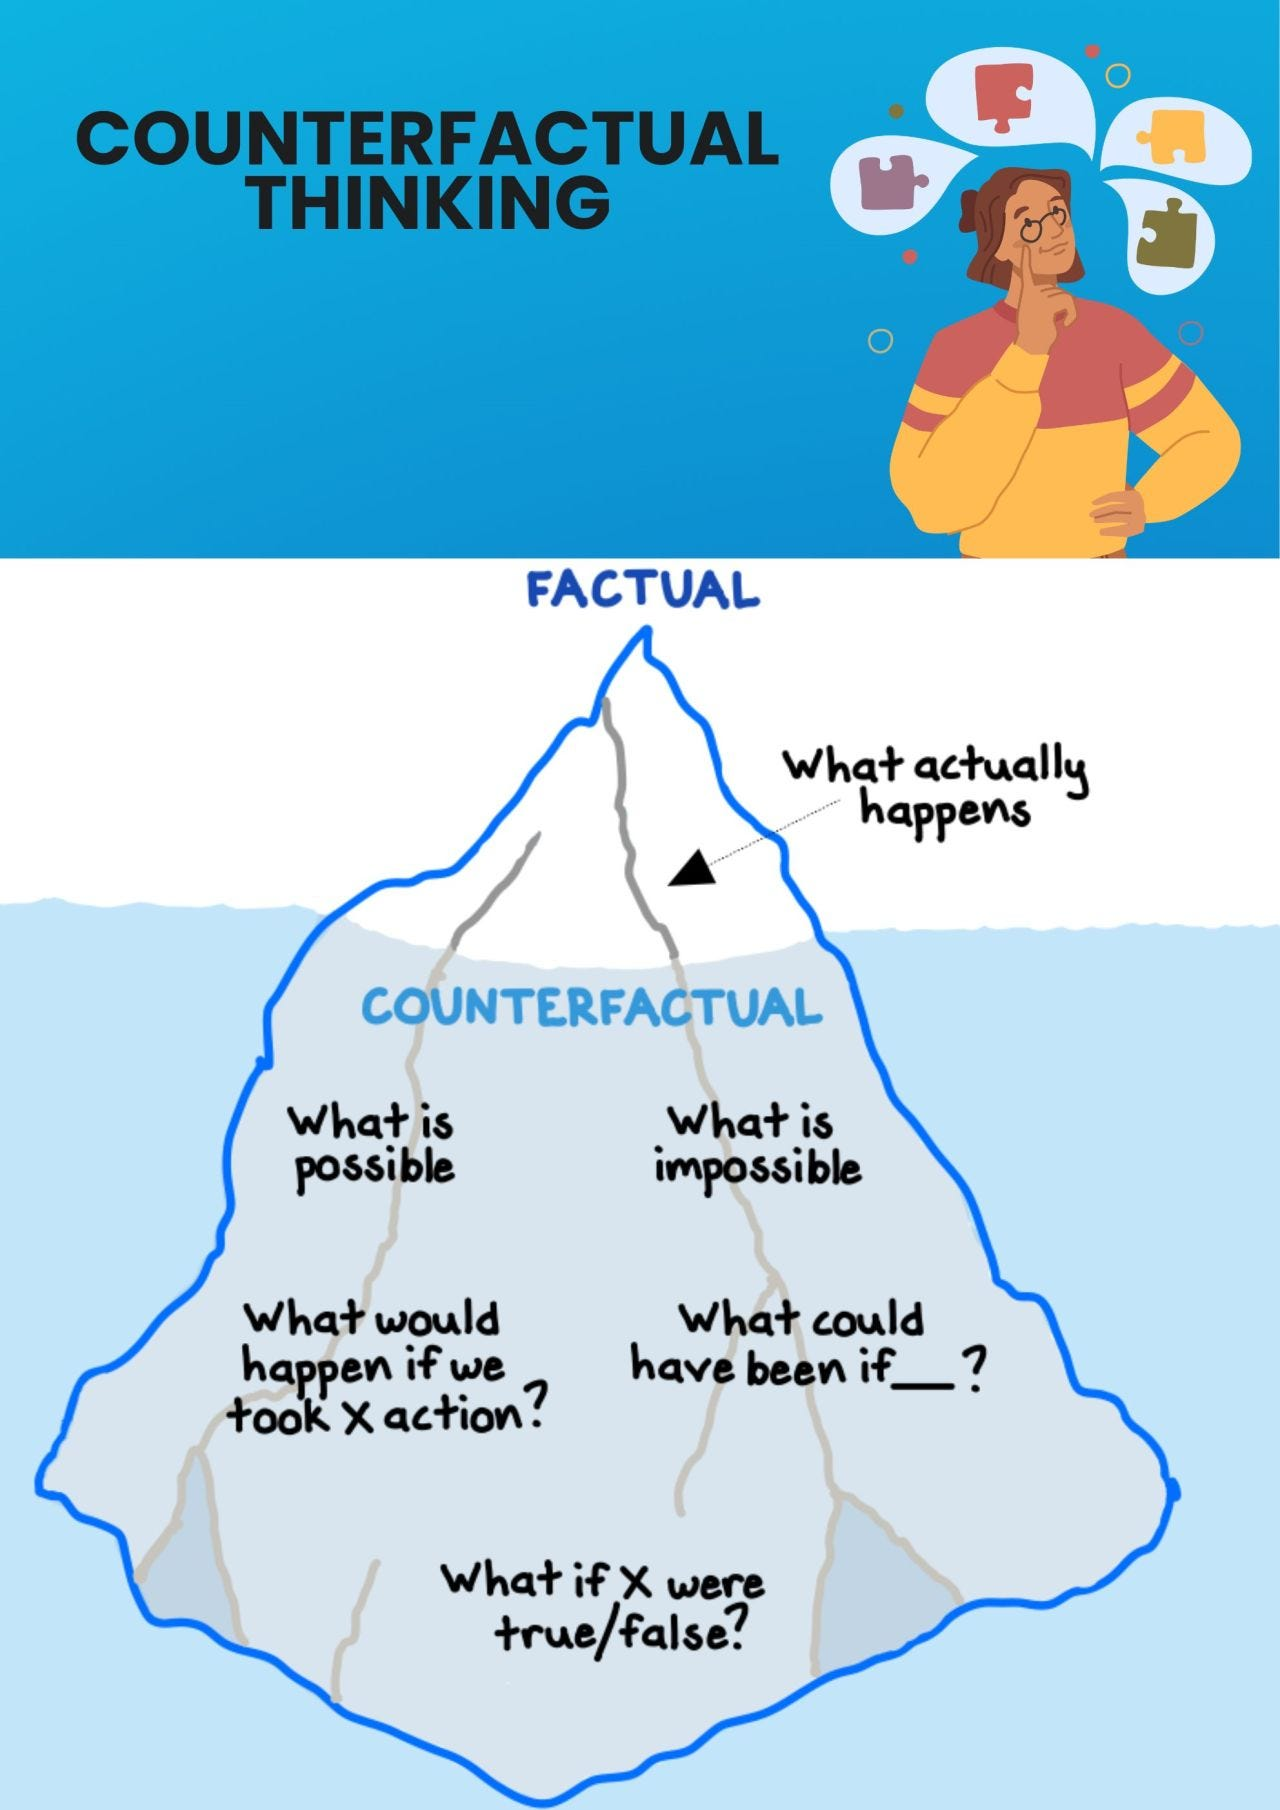
\includegraphics[height=0.72\textheight]{figures/s05_1_4.6x4.4.jpg}
    \end{column}
  \end{columns}
\end{frame}

%---------------------------------------------------------------------
%  04 RCTs  (EMBED RCT flowchart)
%---------------------------------------------------------------------
\begin{frame}{\numbadge{04}\ \ Randomized Experiments (RCTs)}
  \begin{columns}[T]
    \begin{column}{0.5\textwidth}
      \textbf{\color{qrnavy}Key Components}
      \begin{itemize}\small
        \item \textbf{Treatment:} condition applied to experimental units.
        \item \textbf{Control group:} valid counterfactual.
        \item \textbf{Random assignment:} treatment determined by chance.
      \end{itemize}
    \end{column}
    \begin{column}{0.5\textwidth}
      \textbf{\color{qrnavy}Why randomize?}
      \begin{itemize}\small
        \item Creates balance between treatment / control groups.
        \item Groups identical ``on average'' (observable + unobservable characteristics).
        \item Only difference is the treatment effect.
      \end{itemize}
    \end{column}
  \end{columns}
  \vspace{0.3em}
  \begin{center}
    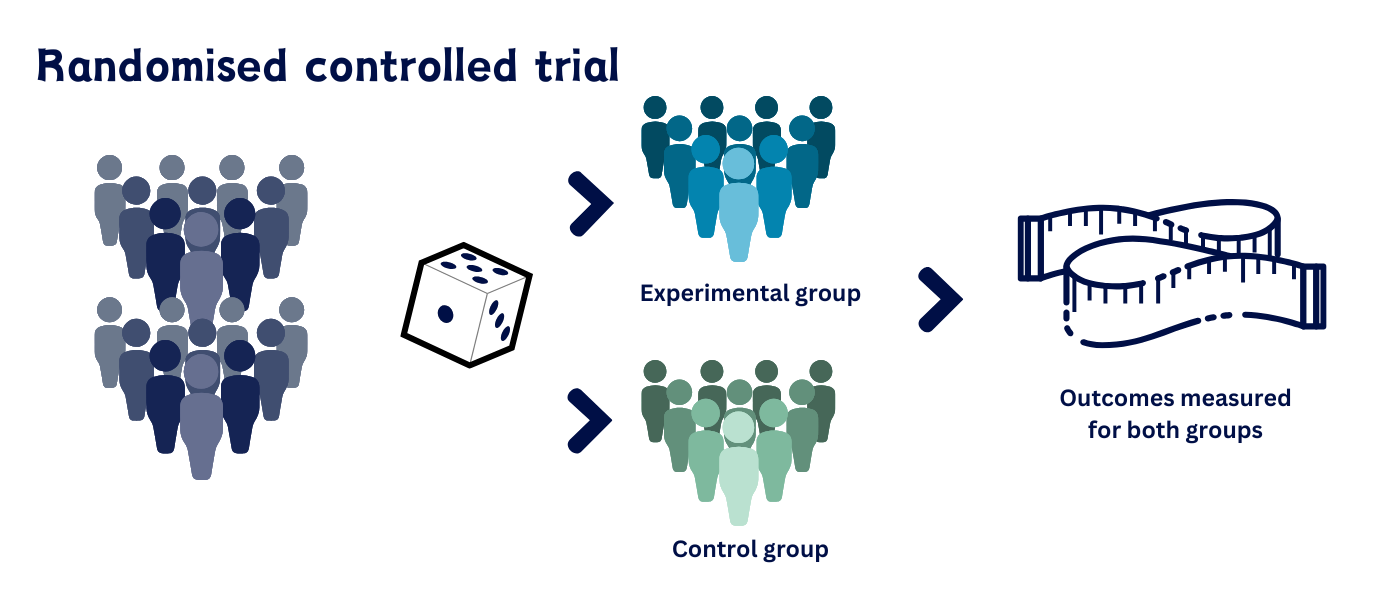
\includegraphics[width=0.82\textwidth]{figures/s06_1_7.4x2.7.png}
  \end{center}
\end{frame}

%---------------------------------------------------------------------
%  05 Problems with Experiments
%---------------------------------------------------------------------
\begin{frame}{\numbadge{05}\ \ Problems with Experiments}
  \begin{itemize}
    \item \textbf{Selection bias:} voluntary participation creates unrepresentative samples.
    \item \textbf{Placebo effects:} responding to attention rather than treatment.
    \item \textbf{Hawthorne effects:} acting differently when observed.
    \item \textbf{External validity:} may not reflect real-world conditions.
  \end{itemize}
  \vspace{0.5em}
  \begin{keybox}[Remedies]
    \begin{itemize}
      \item Double-blind experiments.
      \item Balance checking on pre-treatment variables.
    \end{itemize}
  \end{keybox}
\end{frame}

%---------------------------------------------------------------------
%  06 Sampling (1)  (EMBED population -> sample figure)
%---------------------------------------------------------------------
\begin{frame}{\numbadge{06}\ \ Sampling (1)}
  \begin{keybox}
    Making inferences from a small group to a larger population.
    \begin{itemize}
      \item \textbf{Population:} complete set we want to learn about.
      \item \textbf{Sample:} part we actually collect data from.
    \end{itemize}
  \end{keybox}
  \vspace{0.2em}
  \begin{columns}[T]
    \begin{column}{0.56\textwidth}
      \textbf{\color{qrnavy}Good sampling}
      \begin{itemize}\footnotesize
        \item \textbf{Simple Random Sampling (SRS):} everyone has an equal chance of being selected.
        \item \textbf{Stratified Sampling:} divide the population into groups, then randomly sample within each group.
        \item \textbf{Multistage Sampling:} sample in stages (e.g., cities $\rightarrow$ neighborhoods $\rightarrow$ households).
      \end{itemize}
    \end{column}
    \begin{column}{0.44\textwidth}
      \centering
      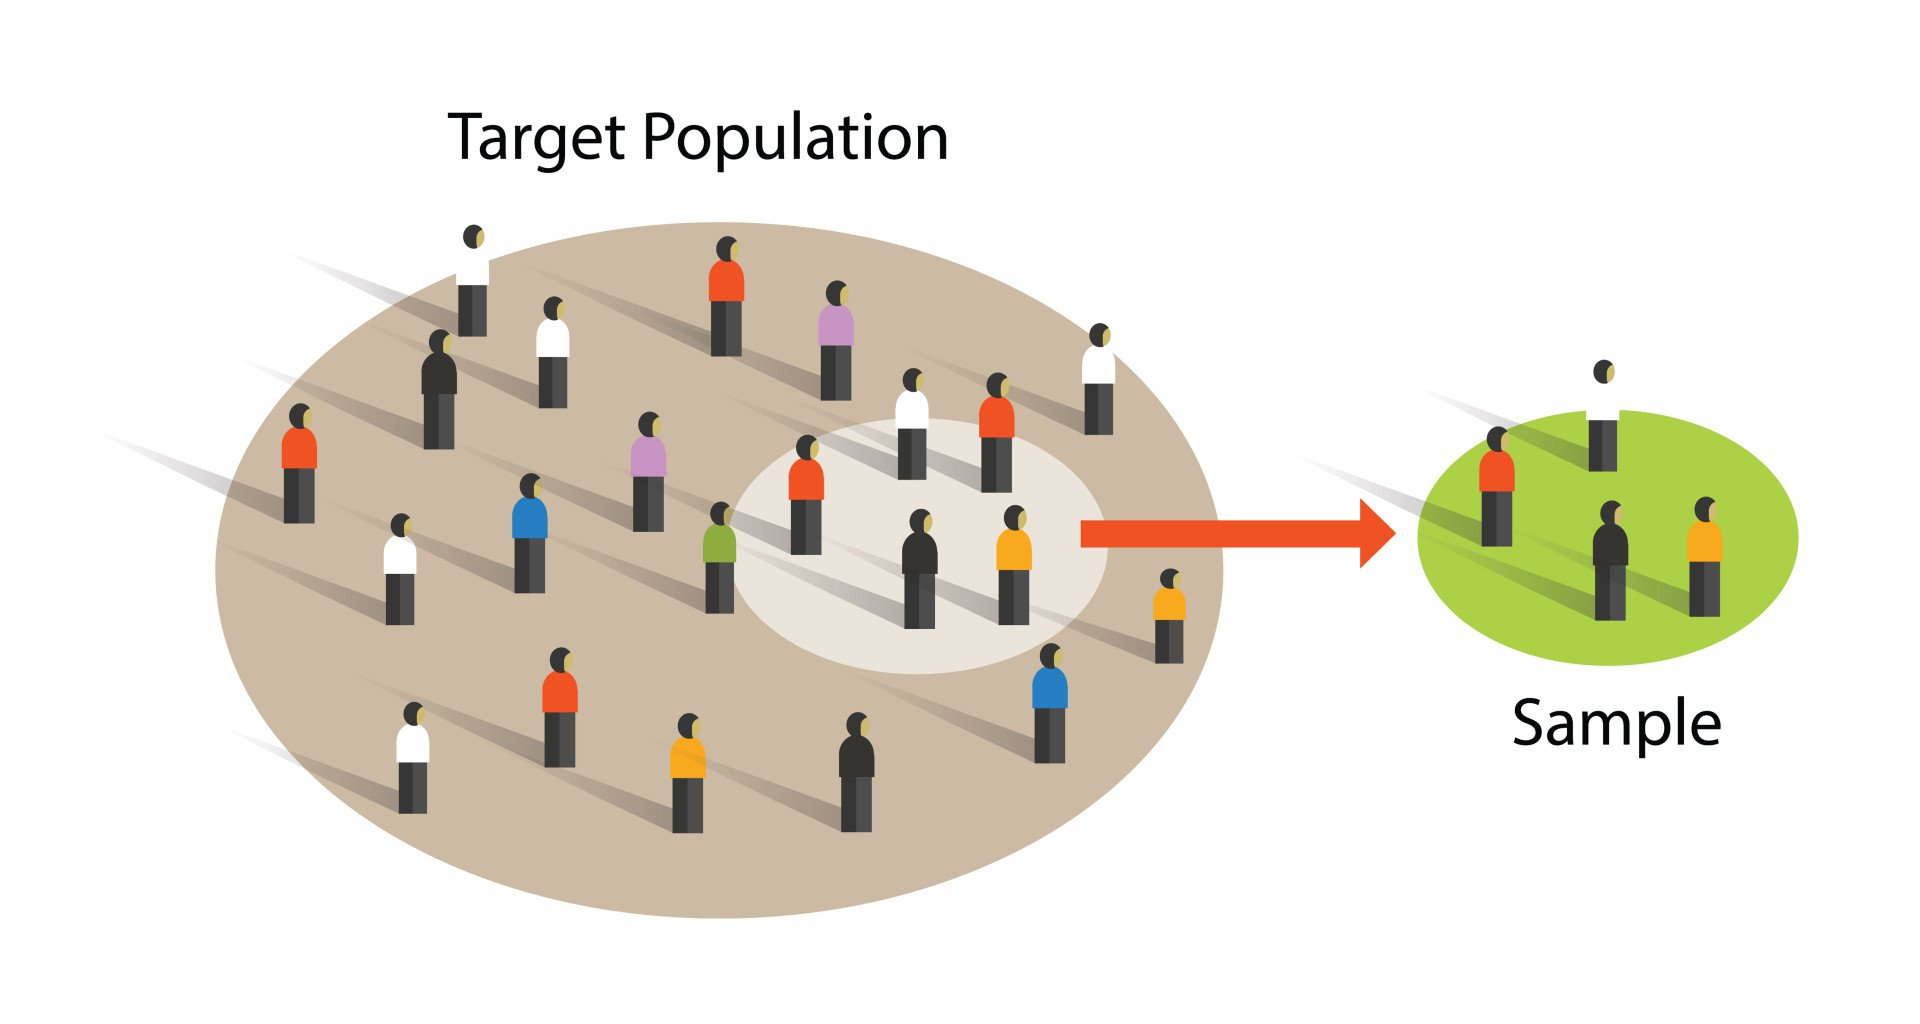
\includegraphics[width=\textwidth]{figures/s08_1_4.7x2.6.jpg}
    \end{column}
  \end{columns}
\end{frame}

%---------------------------------------------------------------------
%  06 Sampling (2)  (EMBED sampling-bias cartoon)
%---------------------------------------------------------------------
\begin{frame}{\numbadge{06}\ \ Sampling (2)}
  \begin{columns}[T]
    \begin{column}{0.52\textwidth}
      \textbf{\color{qrnavy}Bad sampling}
      \begin{itemize}
        \item \textbf{Convenience:} just picking whoever's easy to reach.
        \item \textbf{Voluntary response:} letting people self-select into your study.
      \end{itemize}
      \vspace{0.5em}
      \begin{keybox}[Key Principle]
        The sample needs to be representative of the target population!
      \end{keybox}
    \end{column}
    \begin{column}{0.48\textwidth}
      \centering
      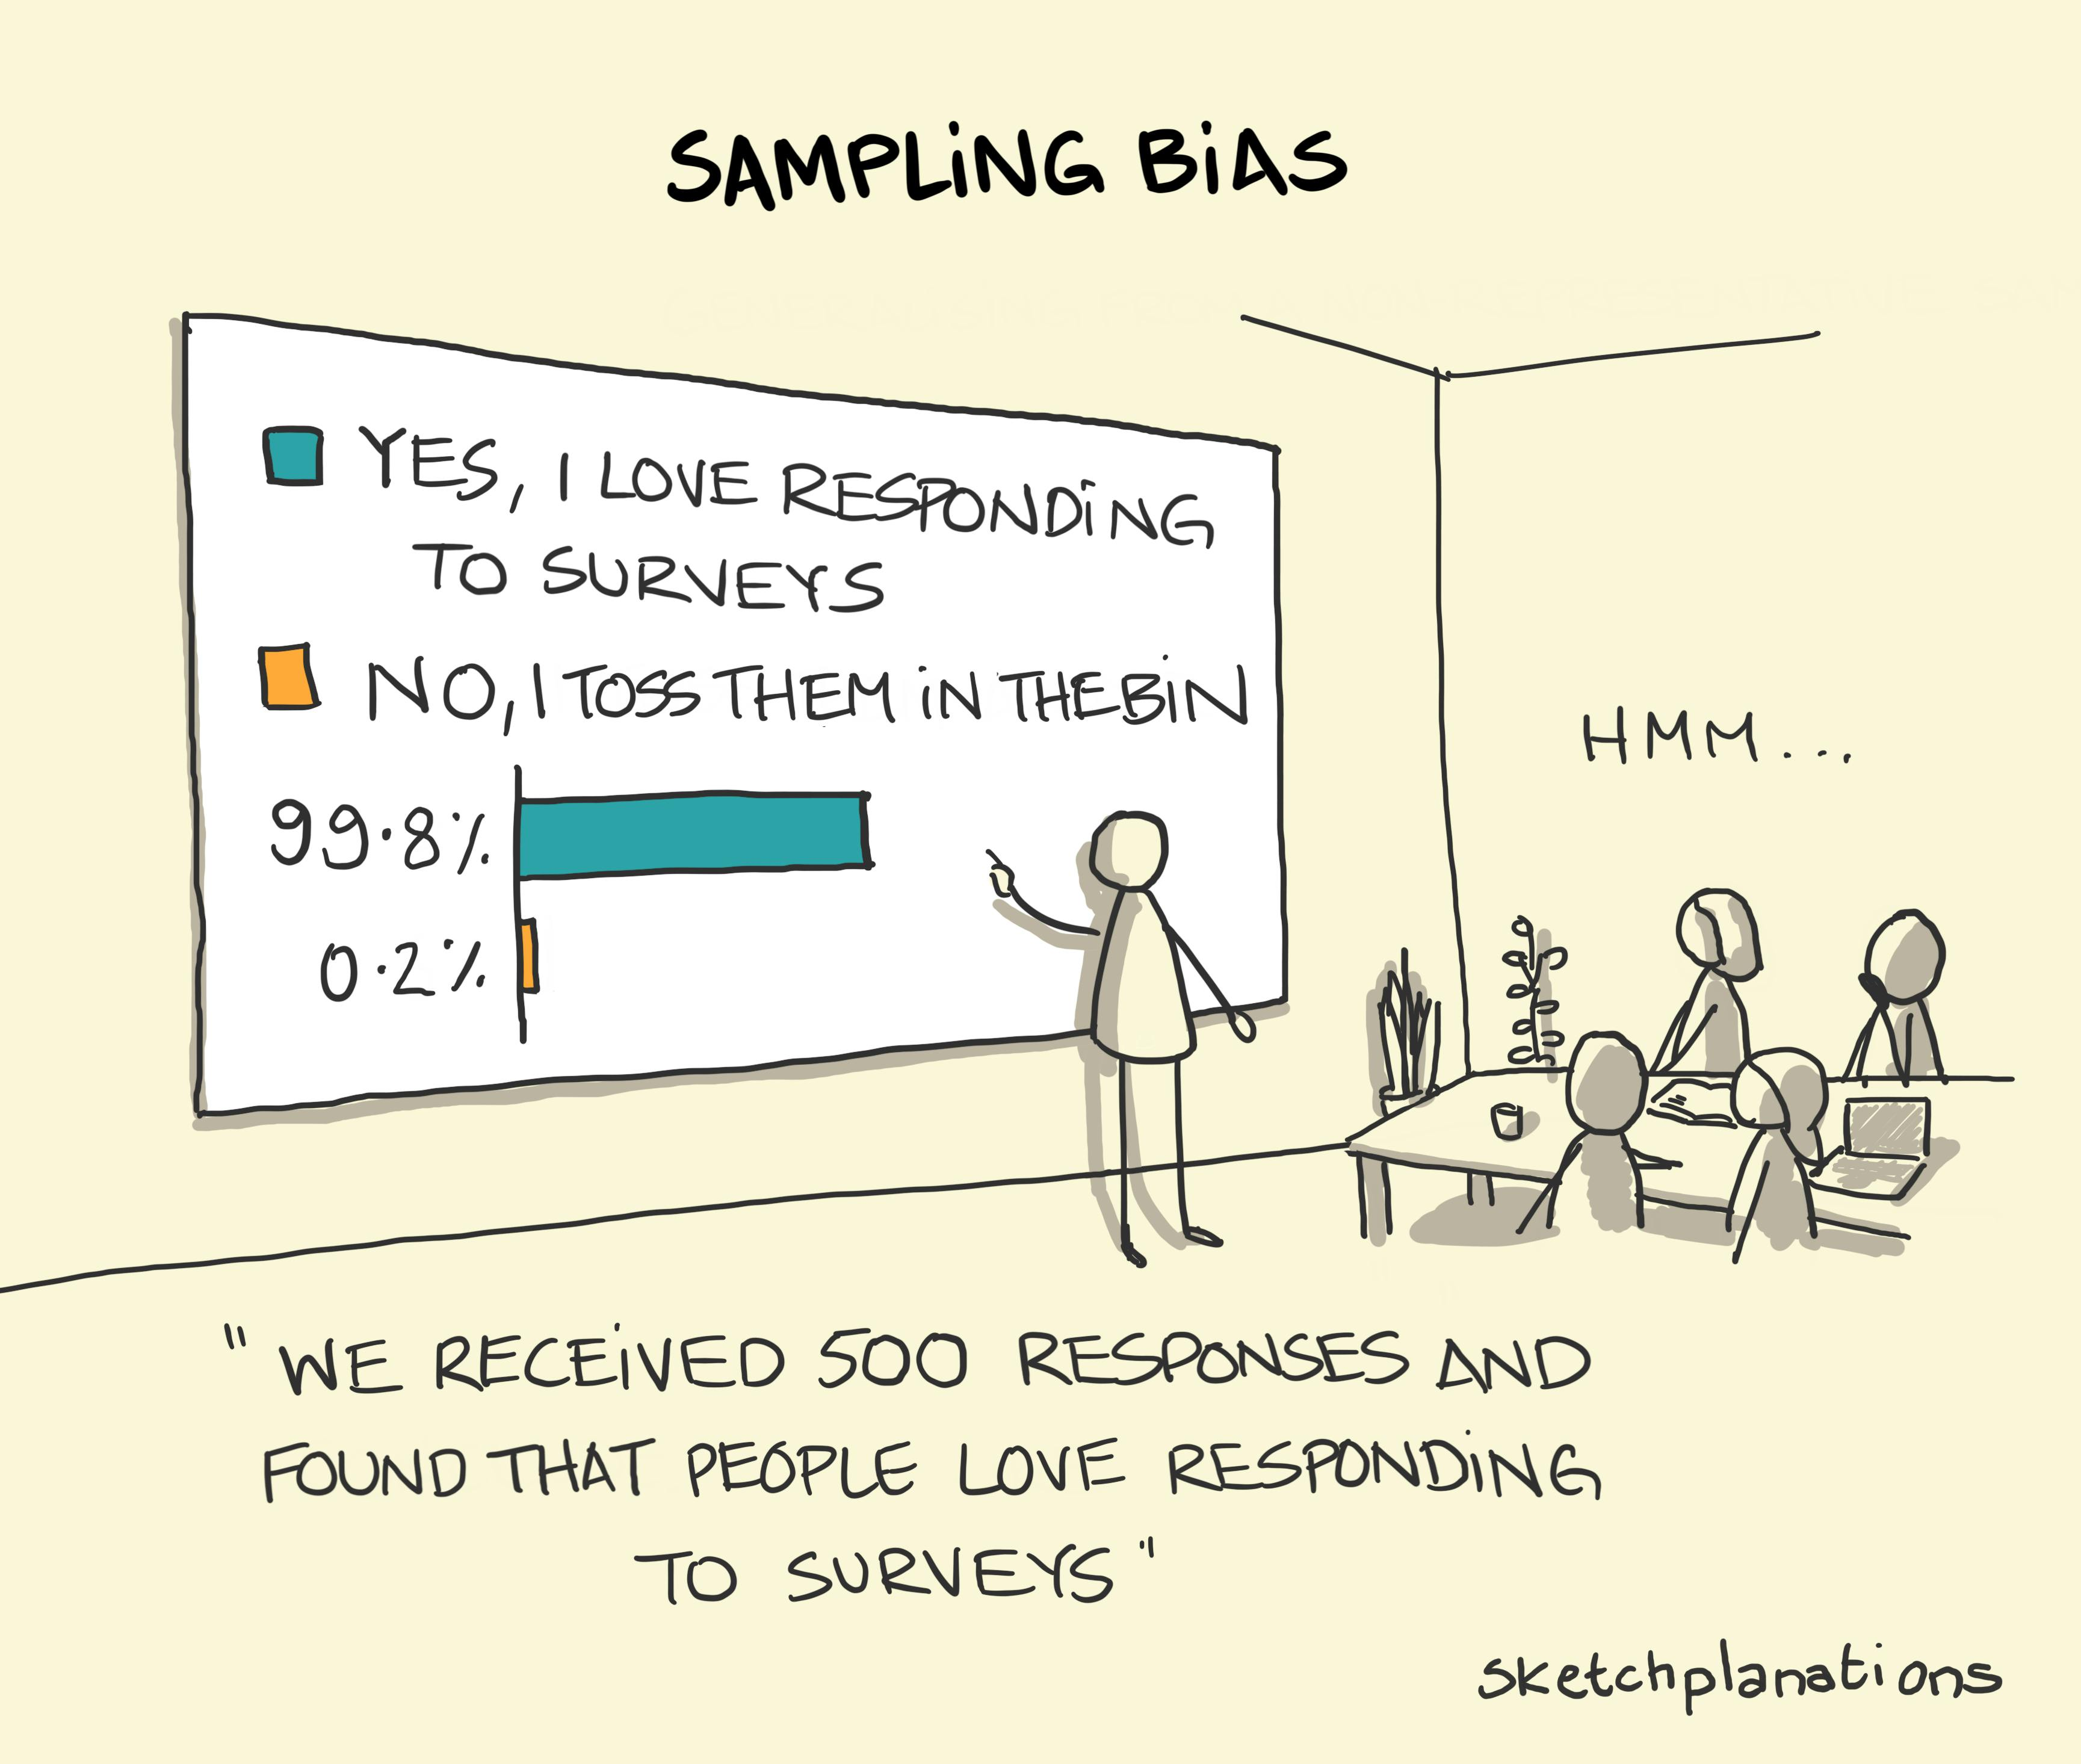
\includegraphics[height=0.66\textheight]{figures/s09_2_6.3x5.4.jpg}
    \end{column}
  \end{columns}
\end{frame}

%---------------------------------------------------------------------
%  07 Survey Cautions
%---------------------------------------------------------------------
\begin{frame}{\numbadge{07}\ \ Survey Cautions}
  \begin{itemize}
    \item \textbf{Undercoverage:} missing population groups.
    \item \textbf{Nonresponse:} people don't participate.
    \item \textbf{Response bias:} systematic incorrect responses.
    \item \textbf{Question wording:} the most important influence on responses.
  \end{itemize}
  \vspace{0.4em}
  \begin{tcolorbox}[colback=qrlight,colframe=qrblue,arc=2pt]
    \small ``Should we reduce government spending?'' \quad vs.\ \quad
    ``Should we cut funding for education and healthcare?''
  \end{tcolorbox}
  \vspace{0.3em}
  \begin{center}
    \textbf{\color{qrred}Always pilot test surveys!}
  \end{center}
\end{frame}

%---------------------------------------------------------------------
%  Transition to RStudio
%---------------------------------------------------------------------
{\setbeamertemplate{footline}{}
\begin{frame}
  \vfill
  \centering
  {\color{qrnavy}\Huge\bfseries RStudio Practice}\\[0.8em]
  {\color{qrblue}\large School Data: Summaries, ``Top'' Schools \& Regression}\\[0.4em]
  {\color{qrgray} See \texttt{Lab4.Rmd} / \texttt{Lab4\_0924.R}}
  \vfill
\end{frame}
}

\end{document}
